\documentclass[tikz,border=10pt]{standalone}


\begin{document}
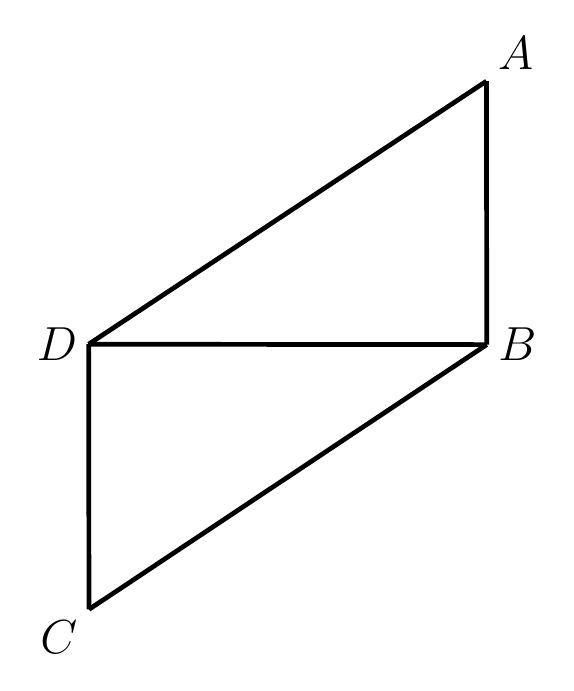
\begin{tikzpicture}[line join=round, line width=1.7pt]
\coordinate (A) at (2.524,3.365);
\coordinate (B) at (2.528,0.019);
\coordinate (C) at (-2.524,-3.344);
\coordinate (D) at (-2.528,0.024);

  
  \draw (A) -- (B);   
  \draw (B) -- (D);   
  \draw (D) -- (A);   
  \draw (D) -- (C);   
  \draw (C) -- (B);   
  
  \node[above right] at (A) {\fontsize{17.5}{21}\selectfont $A$};
  \node[right] at (B) {\fontsize{17.5}{21}\selectfont $B$};
  \node[below left] at (C) {\fontsize{17.5}{21}\selectfont $C$};
  \node[left] at (D) {\fontsize{17.5}{21}\selectfont $D$};
\end{tikzpicture}
\end{document}